\documentclass[11pt]{article}
\usepackage[margin=1in]{geometry}
\usepackage{graphicx}
\usepackage{booktabs}
\usepackage{amsmath}
\usepackage{amssymb}
\usepackage{xcolor}
\usepackage[hidelinks]{hyperref}
\usepackage{caption}
\captionsetup{font=small}

\title{\vspace{-2.5em}Sparks in the det6/det7 run: do they correlate with each other,
and do they cross-talk into M3?\\\large (\texttt{mx17\_det6\_det7\_overnight\_6-26-26 /
long\_run})}
\author{MX17 cosmic-bench QA}
\date{\today}

\begin{document}
\maketitle
\vspace{-1.5em}

\section{Setup}
This run reads out \emph{two} detectors under test through the shared DAQ: det6 (FEU3/4)
and det7 (FEU6/8), plus the M3 reference telescope (FEU1). A spark $=$ that detector
fires $>50$ strips. We ask two things: (1) do det6 and det7 sparks correlate event by
event, and (2) does a spark in \emph{either} detector inject excess noise into the shared
M3 readout (the cross-talk confirmed for det3, companion note
\texttt{det3\_spark\_analysis} Q2c)? For (2) we decoded the raw M3 \texttt{.fdf} (pulled
from lxplus, \texttt{DataReader \dots analyse}) and joined on \texttt{evn} (100\,\% match
in a 43\,136-event window).

\section{det6 and det7 sparks are moderately correlated --- a shared muon, not a glitch}
Over 71\,705 events, det6 sparks 24.0\,\% and det7 31.0\,\% of the time. They are
positively correlated but far from lock-step (Fig.~\ref{fig:corr}):
%
\begin{table}[h]\centering\small
\begin{tabular}{lrr}
\toprule
 & det7 spark & det7 quiet\\
\midrule
det6 spark & 9\,669 & 7\,536\\
det6 quiet & 12\,578 & 41\,922\\
\bottomrule
\end{tabular}
\quad
\begin{tabular}{lr}
\toprule
$P(\text{det7}\,|\,\text{det6 spark})$ & 56.2\,\%\\
$P(\text{det7}\,|\,\text{det6 quiet})$ & 23.1\,\% \;($2.4\times$)\\
$P(\text{det6}\,|\,\text{det7 spark})$ & 43.5\,\%\\
$P(\text{det6}\,|\,\text{det7 quiet})$ & 15.2\,\% \;($2.9\times$)\\
odds ratio / $\phi$ & 4.3 / 0.31\\
coincidences vs chance & $9669/5338=1.8\times$\\
\bottomrule
\end{tabular}
\end{table}
%
So when one detector sparks the other is $\sim2.4$--$2.9\times$ more likely to spark, and
double-sparks occur $1.8\times$ above chance --- a real but \textbf{moderate} correlation
($\phi=0.31$). It is \emph{not} a global HV/DAQ glitch: that would force near-total
coincidence ($\phi\to1$), whereas here most sparks are single-detector (7\,536 det6-only,
12\,578 det7-only vs 9\,669 both). The moderate excess is what a \textbf{shared muon}
produces: det6 and det7 are stacked in the same telescope, a cosmic crosses both, and each
sparks muon-induced (det7 shows a $5.9\times$ muon enhancement, companion note) --- so
their sparks partially coincide through the common muon, without either driving the other.
(A small inter-detector DAQ-coupling contribution cannot be excluded, but Sec.~3 shows the
shared-readout coupling is only a few-cluster noise effect --- far too weak to fake a
$50$-strip spark.)

\begin{figure}[h]\centering
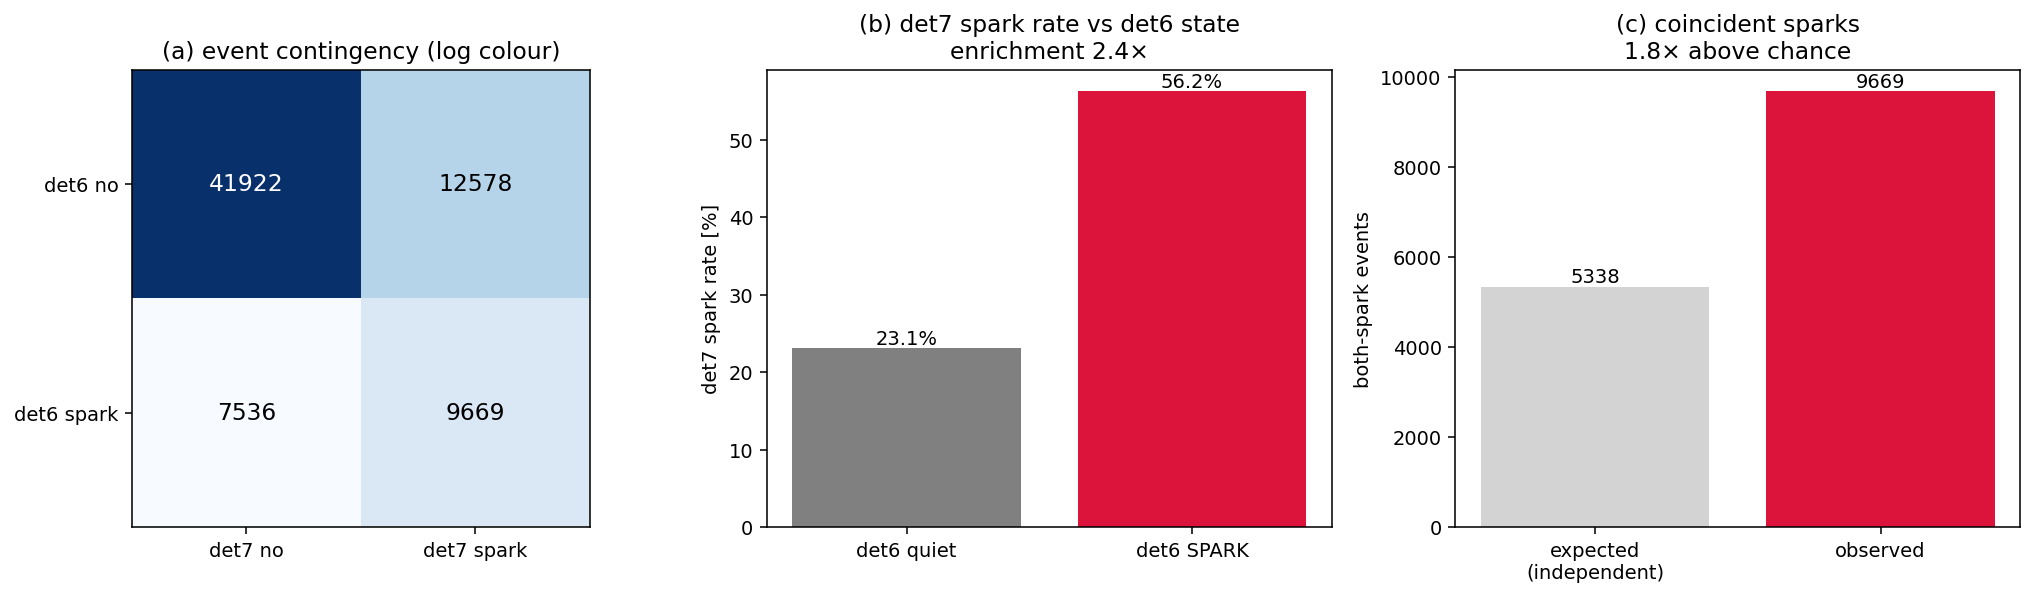
\includegraphics[width=\textwidth]{fig_correlation.png}
\caption{\textbf{det6 $\leftrightarrow$ det7 spark correlation.} (a) event contingency
(log colour); (b) det7 spark rate is $2.4\times$ higher when det6 sparks; (c) coincident
double-sparks occur $1.8\times$ above the independent expectation.}
\label{fig:corr}
\end{figure}

\section{M3 cross-talk confirmed --- with a clean dose-response}
Accounting for \emph{both} detectors (``our spark'' $=$ det6 or det7 fires), the M3/FEU1
result reproduces det3 and adds a decisive causal handle (Fig.~\ref{fig:xt}):
%
\begin{itemize}\setlength\itemsep{0.1em}
  \item \textbf{M3 is not knocked out}: it never fires its own spark
        (\texttt{MGv2\_Spark}$=0$ in all 51\,916 decoded events) and drops \emph{no}
        triggers (100\,\% present).
  \item \textbf{Excess M3 clusters when we spark}: $11.1$ vs $8.8$ per event
        (\textbf{+26\,\%}) for either-detector sparks.
  \item \textbf{Dose-response}: neither $8.8\to$ one detector $\sim\!10.1\to$
        \textbf{both $12.9$} ($+47\,\%$). The more the shared DAQ discharges, the more
        spurious M3 clusters appear --- a monotonic dose-response is exactly what a
        cross-talk (noise-injection) mechanism predicts, and hard to explain any other way.
\end{itemize}
%
This confirms, on an independent run and with two spark sources, the det3 picture: sparks
do not make M3 discharge or lose triggers, but they inject low-level noise into the shared
readout in proportion to how much is sparking. That noise adds spurious hits that spoil the
M3 straight-line fit, explaining the elevated ``no clean M3 track'' rate in spark events.

\begin{figure}[h]\centering
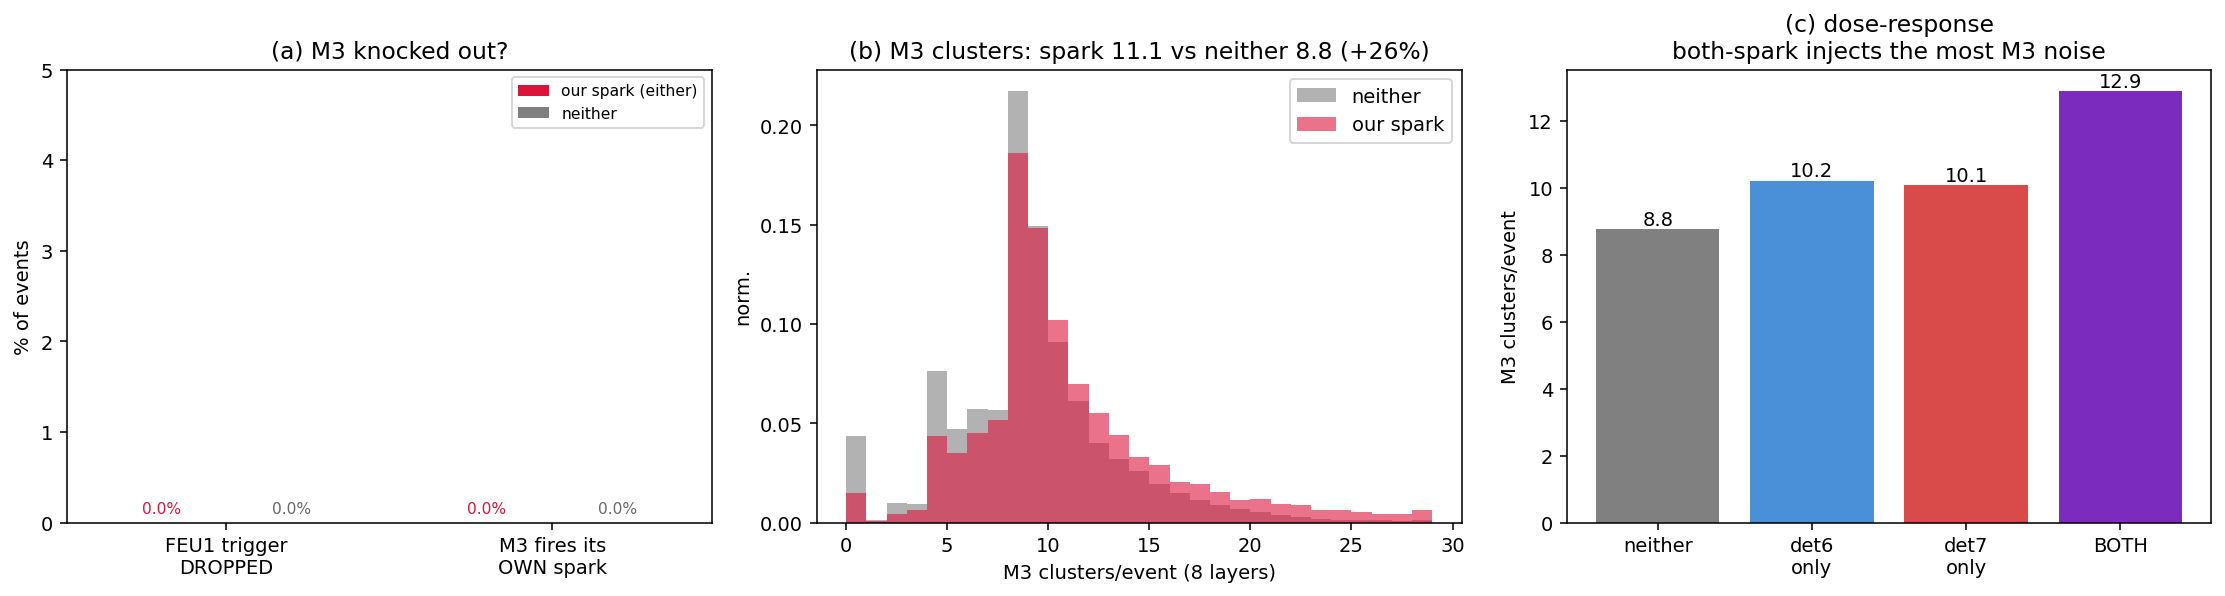
\includegraphics[width=\textwidth]{fig_crosstalk_d67.png}
\caption{\textbf{M3 cross-talk (both detectors).} (a) M3 never drops a trigger nor sparks
(both 0\,\%); (b) $+26\,\%$ M3 clusters when either detector sparks; (c) \textbf{dose-response}
--- neither $\to$ one $\to$ both injects progressively more M3 noise.}
\label{fig:xt}
\end{figure}

\section{Takeaways}
\begin{itemize}\setlength\itemsep{0.15em}
  \item det6 and det7 sparks correlate \textbf{moderately} ($2.4$--$2.9\times$ conditional,
        $1.8\times$ coincidence, $\phi=0.31$) --- consistent with a \textbf{shared muon}
        through the stacked detectors, not a global HV/DAQ glitch (which would be near-total)
        and not a strong inter-detector discharge coupling.
  \item The \textbf{M3 cross-talk is confirmed} on this run counting both detectors'
        sparks, with a clean \textbf{dose-response} (more sparking $\to$ more M3 noise) that
        nails the causal direction. M3 itself never discharges or drops triggers.
  \item Consistent with det3: the cross-talk is a mild, shared-DAQ noise injection ---
        a grounding/shielding issue, not a physical M3 discharge.
\end{itemize}

\vspace{0.4em}
\footnotesize\noindent\textit{Reproduce:} \texttt{correlate\_sparks.py} (local, from
combined\_hits) $\to$ \texttt{d67\_events.npz}; FEU1 decoded with
\texttt{cosmic\_bench\_m3\_tracking DataReader config\_d67\_cos.json analyse}; then
\texttt{crosstalk\_feu1\_d67.py}. Numbers in \texttt{correlation.json},
\texttt{crosstalk\_d67.json}.

\end{document}
